\documentclass[12pt,a4paper,portrait]{article}
%\setcounter{secnumdepth}{0}
\usepackage{gensymb}
\usepackage{pdflscape}
\usepackage{amsmath}
\usepackage{amssymb}
\usepackage{enumitem}
\usepackage{graphicx}
\usepackage{subcaption}
\usepackage{multirow}
\usepackage{sansmath}
\usepackage{pst-eucl}
\usepackage{multicol}
\usepackage{csquotes}
% Coding
\usepackage{listings}
\setlength{\parindent}{0pt}
\usepackage[obeyspaces]{url}
% Better inline directory listings
\usepackage{xcolor}
\definecolor{light-gray}{gray}{0.95}
\newcommand{\code}[1]{\colorbox{light-gray}{\texttt{#1}}}
\usepackage{adjustbox}
\usepackage[UKenglish]{isodate}
\usepackage[UKenglish]{babel}
\usepackage{float}
\usepackage[T1]{fontenc}
\usepackage{setspace}
\usepackage{sectsty}
\usepackage{longtable}
\newenvironment{tightcenter}{%
	\setlength\topsep{0pt}
	\setlength\parskip{0pt}
	\begin{center}
	}{%
	\end{center}
}
\captionsetup{width=\textwidth}
\usepackage{mbenotes} % to print table notes!
\usepackage{alphalph} % For extended counters!
% usage: \tabnotemark[3]\cmsp\tabnotemark[4]
\usepackage[colorlinks=true,linkcolor=blue,urlcolor=black,bookmarksopen=true]{hyperref}
\sectionfont{%			            % Change font of \section command
	\usefont{OT1}{phv}{b}{n}%		% bch-b-n: CharterBT-Bold font
	\sectionrule{0pt}{0pt}{-5pt}{3pt}}
\subsectionfont{
	\usefont{OT1}{phv}{b}{n}}
\newcommand{\MyName}[1]{ % Name
	\usefont{OT1}{phv}{b}{n} \begin{center}of {\LARGE  #1}\end{center}
	\par \normalsize \normalfont}
\makeatletter
\newcommand\FirstWord[1]{\@firstword#1 \@nil}%
\newcommand\@firstword{}%
\newcommand\@removecomma{}%
\def\@firstword#1 #2\@nil{\@removecomma#1,\@nil}%
\def\@removecomma#1,#2\@nil{#1}
\makeatother

\newcommand{\MyTitle}[1]{ % Name
	\Huge \usefont{OT1}{phv}{b}{n} \begin{center}#1\end{center}
	\par \normalsize \normalfont}
\newcommand{\lag}{\mathcal{L}}
\newcommand{\ham}{\mathcal{H}}
\newcommand{\eq}[1]{Equation \eqref{#1}}
\newcommand{\NewPart}[1]{\section*{\uppercase{#1}}}
\newcommand{\NewSubPart}[1]{\subsection*{\hspace{0.2cm}#1}}
\renewcommand{\baselinestretch}{1.05}
\usepackage[margin=0.2cm]{geometry}
\date{}
\title{Elastic pendula}
\author{Brenton Horne}

\begin{document}
\maketitle

In this document, we will go over classical mechanical problems that involve an elastic pendulum. An elastic pendulum is one whose rod instead of being rigid is an elastic spring. This complicates the calculation by making the length of the pendulum rod variable instead of fixed and adding an extra force to the system (the spring force). Friction forces will be accounted for using linear and quadratic (of velocity) terms. 
\tableofcontents

\section{Preliminaries}
There are a few classical mechanical formalisms we could use to derive the equations of motion for elastic pendulum systems with friction. Newtonian mechanics is one approach, but this approach uses vectors and is unnecessarily complicated. Alternatively, Lagrangian and Hamiltonian mechanics could provide a simpler path to a solution. Of these, Lagrangian mechanics is likely simpler, as using the Hamiltonian approach would require us to write the kinetic energy in terms of generalized momenta ($p_i$), which will take some work. Hamiltonian mechanics usually makes up for this by providing ordinary differential equation (ODE) systems that can be integrated using symplectic methods. These methods minimize the accumulation of errors in the Hamiltonian of the system over time. 

\subsection{Lagrangian formalism}
In Lagrangian mechanics, the equations of motion are the Euler-Lagrange equations, which are in terms of the Lagrangian --- $\lag$ --- which is the kinetic and potential energy difference. These equations can be written, with a dissipative force, as
\begin{align}
	\dfrac{d}{dt}\left(\dfrac{\partial \lag}{\partial \dot{q}_i}\right) - \dfrac{\partial \lag}{\partial q_i} &= Q_i. \label{ELD}
\end{align}

Where $Q_i$ is the generalized dissipative force, which is defined as
\begin{align}
	Q_i &= \sum_{j} \vec{F}_{D,j} \cdot \hat{e}_{j,i}.\label{GDF}
\end{align}

Where $\vec{F}_{D,j}$ is the dissipative force vector for particle $j$. In \eq{GDF}, $\hat{e}_{j,i}$ is the generalized basis vector of particle $j$ and generalized coordinate $q_i$. In this case, our generalized coordinates $q_i$ would consist of $\theta$ and $z$. The generalized basis vectors are defined as
\begin{align*}
	\hat{e}_{j,i} &= \dfrac{\partial \vec{r}_j}{\partial q_i}.
\end{align*}
 
\subsection{Hamiltonian formalism}
As for the Hamiltonian formalism, the equations of motion there are

\begin{align}
	\dot{q}_i &= \dfrac{\partial \ham}{\partial p_i} \label{qdoti}\\
	\dot{p}_i &= -\dfrac{\partial \ham}{\partial q_i} + Q_i. \label{pdoti}
\end{align}

Where $\ham$ is the kinetic energy plus potential energy. 

\section{Single elastic pendulum with friction}
Say we have a mass $m$ attached to a spring of rest length $l$. Suppose we call the displacement from rest $z$. That way the length of the spring is $l(t) = l + z$. Let us measure  $\theta$ clockwise from the positive x-axis.

\subsection{Position and velocity}
The Cartesian coordinates of the pendulum bob are defined as

\begin{align*}
	x &= (l+z)\cos{\theta} &\implies \dot{x} &= \dot{z}\cos{\theta} - (l+z)\dot{\theta}\sin{\theta}\\
	y &= (l+z)\sin{\theta} &\implies \dot{y} &= \dot{z}\sin{\theta} + (l+z)\dot{\theta}\cos{\theta}.\\
\end{align*}

Velocity is given by

\begin{align*}
	\vec{v} &= \begin{bmatrix}
		\dot{z}\cos{\theta} - (l+z)\dot{\theta}\sin{\theta} \\
		\dot{z}\sin{\theta} + (l+z)\dot{\theta}\cos{\theta}
	\end{bmatrix}\\
	|\vec{v}|^2 &= |\vec{v}|^2 \\
	&= \dot{x}^2+\dot{y}^2 \\
	&= \left[\dot{z}\cos{\theta} - (l+z)\dot{\theta}\sin{\theta}\right]^2 + \left[\dot{z}\sin{\theta} + (l+z)\dot{\theta}\cos{\theta}\right]^2 \\
	&= \dot{z}^2 \cos^2{\theta} + (l+z)^2\dot{\theta}^2\sin^2{\theta} - 2\dot{z}\dot{\theta}(l+z)\cos{\theta}\sin{\theta} + \dot{z}^2\sin^2{\theta} + (l+z)^2\dot{\theta}^2\cos^2{\theta} + 2\dot{z}\dot{\theta}(l+z)\sin{\theta}\cos{\theta} \\
	&= \dot{z}^2 + (l+z)^2\dot{\theta}^2\\
\therefore |\vec{v}| &= \sqrt{|\vec{v}|^2}\\
	&= \sqrt{\dot{z}^2+(l+z)^2\dot{\theta}^2}.
\end{align*}

\subsection{Generalized basis vector}
Next we will calculate $\dfrac{\partial \vec{r}}{\partial q_i}$

\begin{align*}
	\dfrac{\partial \vec{r}}{\partial \theta} &= (l+z)\begin{bmatrix}
		-\sin{\theta} \\
		\cos{\theta}
	\end{bmatrix} \\
	\dfrac{\partial \vec{r}}{\partial z} &= \begin{bmatrix}
		\cos{\theta} \\
		\sin{\theta}
	\end{bmatrix}.
\end{align*}

\subsection{Kinetic energy}
Hence the kinetic energy is
\begin{align*}
	T &= \dfrac{m|\vec{v}|^2}{2} \\
	&= \dfrac{m}{2} \left[\dot{z}^2 + (l+z)^2\dot{\theta}^2\right].
\end{align*}

\subsection{Potential energy}
As for the potential energy, it will have two components: a spring component,
\begin{align*}
	V_S &= \dfrac{kz^2}{2};
\end{align*}

and a graphical component,
\begin{align*}
	V_G &= mgy \\
	&= mg(l+z)\sin{\theta}.
\end{align*}

Therefore the total potential energy is
\begin{align*}
	V &= V_S + V_G \\
	&= \dfrac{kz^2}{2} + mg(l+z)\sin{\theta}.
\end{align*}

\subsection{Lagrangian}
Hence the Lagrangian is
\begin{align*}
	\lag &= T - V \\
	&= \dfrac{m}{2} \left[\dot{z}^2 + \dot{\theta}^2(l+z)^2\right] - \dfrac{kz^2}{2} - mg(l+z)\sin{\theta}.
\end{align*}

\subsection{Dissipative forces}
What dissipative forces should be included? Let us include linear and quadratic in velocity terms to account for air resistance and other forms of friction. 

\begin{align*}
	\vec{F}_D &= -b\vec{v} - c|\vec{v}|\vec{v}.
\end{align*}

We have already calculate the components of the velocity vector---they are $\dot{x}$ and $\dot{y}$, respectively. 

\begin{align*}
	\vec{v} &= \begin{bmatrix}
		\dot{z}\cos{\theta} - (l+z)\dot{\theta}\sin{\theta} \\
		\dot{z}\sin{\theta} + (l+z)\dot{\theta}\cos{\theta}
	\end{bmatrix}\\
	|\vec{v}| &= \sqrt{|\vec{v}|^2}\\
	&= \sqrt{\dot{z}^2+(l+z)^2\dot{\theta}^2}.
\end{align*}

To calculate, $Q_i$ we must find $\vec{v} \cdot \dfrac{\partial \vec{r}}{\partial q_i}$

\begin{align*}
	\vec{v} \cdot \dfrac{\partial \vec{r}}{\partial \theta} &= \begin{bmatrix}
		\dot{z}\cos{\theta} - (l+z)\dot{\theta}\sin{\theta} \\
		\dot{z}\sin{\theta} + (l+z)\dot{\theta}\cos{\theta}
	\end{bmatrix} \cdot (l+z)\begin{bmatrix}
		-\sin{\theta} \\
		\cos{\theta}
	\end{bmatrix} \\
	&= -\dot{z}(l+z)\cos{\theta} \sin{\theta} + (l+z)^2 \dot{\theta}\sin^2{\theta} + \dot{z}(l+z)\sin{\theta} \cos{\theta} +(l+z)^2\dot{\theta}\cos^2{\theta} \\
	&= (l+z)^2 \dot{\theta} \\
	\vec{v} \cdot \dfrac{\partial \vec{r}}{\partial z} &= \begin{bmatrix}
		\dot{z}\cos{\theta} - (l+z)\dot{\theta}\sin{\theta} \\
		\dot{z}\sin{\theta} + (l+z)\dot{\theta}\cos{\theta}
	\end{bmatrix} \cdot \begin{bmatrix}
		\cos{\theta} \\
		\sin{\theta}
	\end{bmatrix} \\
	&= \dot{z}\cos^2{\theta} - (l+z)\dot{\theta} \sin{\theta}\cos{\theta} + \dot{z}\sin^2{\theta} + (l+z)\dot{\theta}\cos{\theta}\sin{\theta} \\
	&= \dot{z}. 
\end{align*}

Hence $Q_i$ is

\begin{align*}
	Q_{\theta} &= -(l+z)^2 \dot{\theta} \left(b+c\sqrt{\dot{z}^2+(l+z)^2\dot{\theta}^2}\right) \\
	Q_z &= -\dot{z}\left(b+c\sqrt{\dot{z}^2+(l+z)^2\dot{\theta}^2}\right).
\end{align*}

\subsection{Left-hand side of \eq{ELD}}
\subsubsection{$\theta$}
As for the LHS of \eq{ELD}, let us work on it for $\theta$ one term at a time
\begin{align*}
	p_{\theta} &= \dfrac{\partial \lag}{\partial \dot{\theta}} \\
	&= m\dot{\theta}(l+z)^2 \\
	\dot{p_{\theta}} &= m\ddot{\theta} (l+z)^2 + 2m\dot{\theta}\dot{z}(l+z) \\
	F_{\theta} &= \dfrac{\partial \lag}{\partial \theta} \\
	&= -mg(l+z)\cos{\theta}.
\end{align*}

Substituting into \eq{ELD} yields
\begin{align*}
	m\ddot{\theta} (l+z)^2 + 2m\dot{\theta}\dot{z}(l+z) - (-mg(l+z)\cos{\theta}) &= -(l+z)^2 \dot{\theta} \left(b+c\sqrt{\dot{z}^2+(l+z)^2\dot{\theta}^2}\right) \\
	m\ddot{\theta} (l+z)^2 + 2m\dot{\theta}\dot{z}(l+z) +mg(l+z)\cos{\theta} &= -(l+z)^2 \dot{\theta} \left(b+c\sqrt{\dot{z}^2+(l+z)^2\dot{\theta}^2}\right) \\
	\ddot{\theta} &= -\dfrac{2\dot{\theta}\dot{z}}{l+z} - \dfrac{g\cos{\theta}}{l+z} -\dfrac{\dot{\theta}}{m} \left(b+c\sqrt{\dot{z}^2+(l+z)^2\dot{\theta}^2}\right). \\
\end{align*}

Let $k'=\dfrac{k}{m}$, $b'=\dfrac{b}{m}$ and $c'=\dfrac{c}{m}$.

\begin{align*}
	\ddot{\theta} &= -\dfrac{2\dot{\theta}\dot{z}}{l+z} - \dfrac{g\cos{\theta}}{l+z} -\dot{\theta} \left(b'+c'\sqrt{\dot{z}^2+(l+z)^2\dot{\theta}^2}\right).
\end{align*}

\subsubsection{$z$}
As for $z$

\begin{align*}
	p_z &= \dfrac{\partial \lag}{\partial \dot{z}} \\
	&= m\dot{z} \\
	\dot{p_z} &= m\ddot{z} \\
	F_z &= \dfrac{\partial \lag}{\partial z} \\
	&= m\dot{\theta}^2(l+z) - kz - mg\sin{\theta}.
\end{align*}

Substituting into \eq{ELD} yields

\begin{align*}
	m\ddot{z} - m\dot{\theta}^2(l+z) + kz + mg\sin{\theta} &= -\dot{z}\left(b+c\sqrt{\dot{z}^2+(l+z)^2\dot{\theta}^2}\right) \\
	\ddot{z} &= \dot{\theta}^2(l+z) - \dfrac{kz}{m} - g\sin{\theta} -\dfrac{\dot{z}}{m}\left(b+c\sqrt{\dot{z}^2+(l+z)^2\dot{\theta}^2}\right).
\end{align*}

Let $k'=\dfrac{k}{m}$, $b'=\dfrac{b}{m}$ and $c'=\dfrac{c}{m}$.

\begin{align*}
	\ddot{z} &= \dot{\theta}^2(l+z) - k'z - g\sin{\theta} -\dot{z}\left(b'+c'\sqrt{\dot{z}^2+(l+z)^2\dot{\theta}^2}\right).
\end{align*}

\subsection{Hamiltonian mechanics}
First, we will rewrite $\vec{v}$ and $|\vec{v}|^2$ in terms of $p_{\theta}$ and $p_z$. 

\begin{align*}
	\vec{v} &= \dfrac{1}{m}\begin{bmatrix}
		p_z\cos{\theta} - \dfrac{p_{\theta}\sin{\theta}}{l+z}\\
		p_z\sin{\theta} + \dfrac{p_{\theta}\cos{\theta}}{l+z}
	\end{bmatrix} \\
	|\vec{v}|^2 &= \dot{z}^2 + (l+z)^2 \dot{\theta}^2 \\
	&= \dfrac{p_z^2}{m^2} + \dfrac{p_{\theta}^2}{m^2(l+z)^2}.
\end{align*}

Hence the kinetic energy is

\begin{align*}
	T &= \dfrac{m}{2} |\vec{v}|^2 \\
	&= \dfrac{p_z^2}{2m} + \dfrac{p_{\theta}^2}{2m(l+z)^2},
\end{align*}

the Hamiltonian is

\begin{align*}
	\ham &= T + V\\
	&= \dfrac{p_z^2}{2m} + \dfrac{p_{\theta}^2}{2m(l+z)^2} + \dfrac{kz^2}{2} + mg(l+z)\sin{\theta},
\end{align*}

and the generalized dissipative forces are

\begin{align*}
	Q_z &= -\dfrac{p_z}{m}\left(b+c\sqrt{\dfrac{p_z^2}{m^2} + \dfrac{p_{\theta}^2}{m^2(l+z)^2}}\right) \\
	Q_{\theta} &= -\dfrac{p_{\theta}}{m} \left(b+c\sqrt{\dfrac{p_z^2}{m^2} + \dfrac{p_{\theta}^2}{m^2(l+z)^2}}\right).
\end{align*}

\subsubsection{$z$}
\begin{align*}
	\dot{z} &= \dfrac{\partial \ham}{\partial p_z} \\
	&= \dfrac{p_z}{m} \\
	\dot{p}_z &= -\dfrac{\partial \ham}{\partial z} + Q_z\\
	&= \dfrac{p_{\theta}^2}{m(l+z)^3} - kz - mg\sin{\theta} + Q_z
\end{align*}

\subsubsection{$\theta$}
\begin{align*}
	\dot{\theta} &= \dfrac{\partial \ham}{\partial p_{\theta}} \\
	&= \dfrac{p_{\theta}}{m(l+z)^2} \\
	\dot{p}_{\theta} &= -\dfrac{\partial \ham}{\partial \theta} + Q_{\theta} \\
	&= -mg(l+z)\cos{\theta} + Q_{\theta}.
\end{align*}

\section{Double pendulum with an elastic second pendulum}
Below we will analyse the double pendulum where the second pendulum is elastic. The rest length of the elastic pendulum is $l$ and its displacement from rest is $x$. Let the masses of the pendulum bobs be $m_1$ and $m_2$, respectively. We will assume the rod/string have no mass. I have tried accounting for it, using a centre of mass approach, in my double pendulum calculation and my experience with simulations is that it does not really make things any more interesting and just adds complexity. 
\begin{figure}[H]
	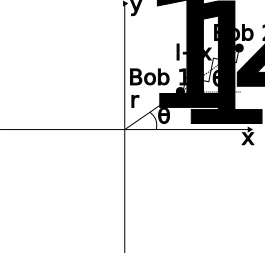
\includegraphics[width=300px]{Double pendulum second elastic.png}
\end{figure}

\subsection{Positions and velocities}
The Cartesian coordinates (and time derivatives thereof) of the first pendulum bob are
\begin{align*}
	x_1 &= r \cos{\theta_1} &\therefore \dot{x}_1 &= -r \dot{\theta}_1 \sin{\theta_1}\\
	y_1 &= r \sin{\theta_1} &\therefore \dot{y}_1 &= r \dot{\theta}_1 \cos{\theta_1}
\end{align*}

As for the second pendulum bob has the coordinates (and time derivatives thereof)
\begin{align*}
	x_2 &= x_1 + (l+z)\cos{\theta_2} & \therefore v_1^2 &= r^2 \dot{\theta}_1^2\\
	&= r \cos{\theta_1} + (l+z)\cos{\theta_2} &\therefore \dot{x}_2 &= -r \dot{\theta}_1 \sin{\theta_1} + \dot{z} \cos{\theta_2}-(l+z)\dot{\theta}_2 \sin{\theta_2}\\
	y_2 &= y_1 + (l+z)\sin{\theta_2} \\
	&= r\sin{\theta_1} + (l+z)\sin{\theta_2} &\therefore \dot{y}_2 &= r \dot{\theta}_1 \cos{\theta_1} + \dot{z} \sin{\theta_2}+(l+z)\dot{\theta}_2 \cos{\theta_2}.
\end{align*}

Hence the velocity of the first pendulum bob is
\begin{align*}
	\vec{v}_1 &= \begin{bmatrix}
		\dot{x}_1 \\
		\dot{y}_1
	\end{bmatrix} & \vec{v}_2 &= \begin{bmatrix}
		\dot{x}_2 \\
		\dot{y}_2
	\end{bmatrix} \\
	&= r\dot{\theta}_1\begin{bmatrix}
		-\sin{\theta_1} \\
		\cos{\theta_1}
	\end{bmatrix} & &= \begin{bmatrix}
		-r \dot{\theta}_1 \sin{\theta_1} + \dot{z} \cos{\theta_2}-(l+z)\dot{\theta}_2 \sin{\theta_2} \\
		r \dot{\theta}_1 \cos{\theta_1} + \dot{z} \sin{\theta_2}+(l+z)\dot{\theta}_2 \cos{\theta_2}
	\end{bmatrix}\\
	|\vec{v}_1| &= r|\dot{\theta}_1|.
\end{align*}
The second pendulum bob has the velocity
\begin{align*}
	|\vec{v}_2|^2 &= \left( -r \dot{\theta}_1 \sin{\theta_1} + \dot{z} \cos{\theta_2}-(l+z)\dot{\theta}_2 \sin{\theta_2}\right)^2 + \left(r \dot{\theta}_1 \cos{\theta_1} + \dot{z} \sin{\theta_2}+(l+z)\dot{\theta}_2 \cos{\theta_2}\right)^2 \\
	&= r^2 \dot{\theta}_1^2 \sin^2{\theta_1}+\dot{z}^2 \cos^2{\theta_2}+(l+z)^2 \dot{\theta}_2^2 \sin^2{\theta_2} - 2r \dot{\theta}_1 \dot{z}\sin{\theta_1}\cos{\theta_2} + 2r (l+z)\dot{\theta}_1 \dot{\theta}_2 \sin{\theta_1}\sin{\theta_2}\\
	&-2\dot{z}(l+z)\dot{\theta}_2 \cos{\theta_2}\sin{\theta_2}+r^2\dot{\theta}_1^2 \cos^2{\theta_1} + \dot{z}^2 \sin^2{\theta_2} + (l+z)^2 \dot{\theta}_2^2\cos^2{\theta_2} + 2r(l+z)\dot{\theta}_1\dot{\theta}_2\cos{\theta_1}\cos{\theta_2}\\
	&+2r\dot{z}\dot{\theta}_1 \cos{\theta_1}\sin{\theta_2}+2\dot{z}\dot{\theta}_2(l+z)\sin{\theta_2}\cos{\theta_2} \\
	&= r^2 \dot{\theta}_1^2 + \dot{z}^2 + (l+z)^2\dot{\theta}_2^2 + 2r\dot{\theta}_1 \dot{z} (\cos{\theta_1}\sin{\theta_2} - \sin{\theta_1}\cos{\theta_2}) + 2r(l+z)\dot{\theta}_1\dot{\theta}_2(\sin{\theta_1}\sin{\theta_2} + \cos{\theta_1}\cos{\theta_2})\\
	&+2\dot{z}\dot{\theta}_2(l+z)(\sin{\theta_2}\cos{\theta_2}-\sin{\theta_2}\cos{\theta_2})\\
	&= r^2 \dot{\theta}_1^2 + \dot{z}^2 + (l+z)^2\dot{\theta}_2^2 + 2r\dot{\theta}_1 \dot{z} \sin{(\theta_2-\theta_1)} + 2r(l+z)\dot{\theta}_1\dot{\theta}_2\cos{(\theta_2 - \theta_1)} \\
	|\vec{v}_2| &= \sqrt{r^2 \dot{\theta}_1^2 + \dot{z}^2 + (l+z)^2\dot{\theta}_2^2 + 2r\dot{\theta}_1 \dot{z} \sin{(\theta_2-\theta_1)} + 2r(l+z)\dot{\theta}_1\dot{\theta}_2\cos{(\theta_2 - \theta_1)}}.
\end{align*}
\subsection{Generalized basis vectors}
The generalized basis vectors for this system are given by
\begin{align*}
	\hat{e}_{1, \theta_1} &= \dfrac{\partial \vec{r}_1}{\partial \theta_1} & \hat{e}_{1, z} &= \dfrac{\partial \vec{r}_1}{\partial z} \\
	&= r\begin{bmatrix}
		-\sin{\theta_1} \\
		\cos{\theta_1}
	\end{bmatrix} & &= 0 \\
	 \hat{e}_{1, \theta_2} &= \dfrac{\partial \vec{r}_1}{\partial \theta_2} & \hat{e}_{2, \theta_1} &= \dfrac{\partial \vec{r}_2}{\partial \theta_1} \\
	 &=0 & &= r\begin{bmatrix}
	 	-\sin{\theta_1} \\
	 	\cos{\theta_1}
	 \end{bmatrix} \\
	\hat{e}_{2, \theta_2} &= \dfrac{\partial \vec{r}_2}{\partial \theta_2} & \hat{e}_{2, z} &=\dfrac{\partial \vec{r}_2}{\partial z}\\
	&= (l+z)\begin{bmatrix}
		-\sin{\theta_2} \\
		\cos{\theta_2}
	\end{bmatrix} & &= \begin{bmatrix}
	\cos{\theta_2}\\
	\sin{\theta_2}
	\end{bmatrix}.
\end{align*}

\subsection{Kinetic energy}
\begin{align*}
	T &= \dfrac{m_1}{2}|\vec{v}_1|^2 + \dfrac{m_2}{2}|\vec{v}_2|^2 \\
	&= \dfrac{m_1r^2 \dot{\theta}_1^2}{2} + \dfrac{m_2(r^2 \dot{\theta}_1^2 + \dot{z}^2 + (l+z)^2\dot{\theta}_2^2 + 2r\dot{\theta}_1 \dot{z} \sin{(\theta_2-\theta_1)} + 2r(l+z)\dot{\theta}_1\dot{\theta}_2\cos{(\theta_2 - \theta_1)})}{2}\\
	&= \dfrac{m_1+m_2}{2}r^2\dot{\theta}_1^2 + \dfrac{m_2(\dot{z}^2 + (l+z)^2\dot{\theta}_2^2 + 2r\dot{\theta}_1[ \dot{z} \sin{(\theta_2-\theta_1)} + (l+z)\dot{\theta}_2\cos{(\theta_2 - \theta_1)}])}{2}.
\end{align*}

\subsection{Potential energy}
\subsubsection{First bob}
For the first bob, the only potential energy is gravitational. 
\begin{align*}
	V_1 &= m_1gy_1 \\
	&= m_1 gr\sin{\theta_1}.
\end{align*}

\subsubsection{Second bob}
For the second bob, there is the spring potential energy and the gravitational potential energy to consider

\begin{align*}
	V_2 &= m_2gy_2 + \dfrac{kz^2}{2} \\
	&= m_2 g(r\sin{\theta_1} + (l+z)\sin{\theta_2}) + \dfrac{kz^2}{2}.
\end{align*}

\subsubsection{Total}
The total potential energy is therefore

\begin{align*}
	V &= V_1 + V_2 \\
	&= m_1 gr\sin{\theta_1} + m_2 g(r\sin{\theta_1} + (l+z)\sin{\theta_2}) + \dfrac{kz^2}{2}.
\end{align*}
\begin{landscape}
\subsection{Lagrangian}
\begin{align*}
	\lag &= T - V \\
	&= \dfrac{m_1+m_2}{2}r^2\dot{\theta}_1^2 + \dfrac{m_2(\dot{z}^2 + (l+z)^2\dot{\theta}_2^2 + 2r\dot{\theta}_1[ \dot{z} \sin{(\theta_2-\theta_1)} + (l+z)\dot{\theta}_2\cos{(\theta_2 - \theta_1)}])}{2} - m_1 gr\sin{\theta_1} \\
	&- m_2 g(r\sin{\theta_1} + (l+z)\sin{\theta_2}) - \dfrac{kz^2}{2}. \\
	&= \dfrac{m_1+m_2}{2}\left(r^2\dot{\theta}_1^2-2gr\sin{\theta_1}\right) + \dfrac{m_2}{2}\left(\dot{z}^2 + (l+z)^2\dot{\theta}_2^2 + 2r\dot{\theta}_1[ \dot{z} \sin{(\theta_2-\theta_1)} + (l+z)\dot{\theta}_2\cos{(\theta_2 - \theta_1)}]-2g(l+z)\sin{\theta_2}\right) - \dfrac{kz^2}{2}.
\end{align*}

\subsection{Euler-Lagrange equations}
\subsubsection{$\theta_1$}
\begin{align*}
	p_{\theta_1} &= \dfrac{\partial \lag}{\partial \dot{\theta}_1} \\
	&= (m_1+m_2)r^2 \dot{\theta}_1 + m_2r[ \dot{z} \sin{(\theta_2-\theta_1)} + (l+z)\dot{\theta}_2\cos{(\theta_2 - \theta_1)}] \\
	\dot{p}_{\theta_1} &= (m_1+m_2)r^2 \ddot{\theta}_1 +  m_2r[ \ddot{z} \sin{(\theta_2-\theta_1)} + \dot{z}(\dot{\theta}_2-\dot{\theta}_1)\cos{(\theta_2-\theta_1)}+ (l+z)\ddot{\theta}_2\cos{(\theta_2 - \theta_1)}- (l+z)\dot{\theta}_2(\dot{\theta}_2-\dot{\theta}_1)\sin{(\theta_2 - \theta_1)}+\dot{z}\dot{\theta}_2\cos{(\theta_2 - \theta_1)}]\\
	&= (m_1+m_2)r^2 \ddot{\theta}_1 +  m_2r[(\ddot{z} -(l+z)\dot{\theta}_2(\dot{\theta}_2-\dot{\theta}_1))\sin{(\theta_2 - \theta_1)}+(\dot{z}(2\dot{\theta}_2-\dot{\theta}_1)+(l+z)\ddot{\theta}_2)\cos{(\theta_2-\theta_1)}]
\end{align*}

Calculating the generalized force for $\theta_1$ (a term taken from \href{https://phys.libretexts.org/Bookshelves/Classical_Mechanics/Graduate_Classical_Mechanics_(Fowler)/04%3A_Hamilton's_Principle_and_Noether's_Theorem/4.05%3A_Generalized_Momenta_and_Forces}{Fowler's Graduate Classical Mechanics})
\begin{align*}
	 F_{\theta_1} &= \dfrac{\partial \lag}{\partial \theta_1} \\
	 &= m_2 r \dot{\theta}_1(\dot{z}\cos{(\theta_2-\theta_1)}\cdot -1 -(l+z)\dot{\theta}_2 \sin{(\theta_2-\theta_1)}\cdot -1) - m_1gr \cos{\theta_1} - m_2gr\cos{\theta_1} \\
	 &= m_2 r\dot{\theta}_1((l+z)\dot{\theta}_2 \sin{(\theta_2-\theta_1)}-\dot{z}\cos{(\theta_2-\theta_1)}) -(m_1+m_2)gr\cos{\theta_1}
\end{align*}

As for the generalized dissipative force, it is

\begin{align*}
	Q_{\theta_1} &= \sum_{j=1}^2 \vec{F}_{D,j} \cdot \hat{e}_{j, \theta_1}.
\end{align*}

Where $j$ refers to the particle (bob 1 or bob 2) under consideration. 

\begin{align*}
	\vec{F}_{D, 1} &= -(b_1+c_1|\vec{v}_1|)\vec{v}_1 \\
	&= -(b_1+c_1r|\dot{\theta}_1|)r\dot{\theta}_1 \begin{bmatrix}
		-\sin{\theta}_1 \\
		\cos{\theta}_1
	\end{bmatrix} \\
	\vec{F}_{D, 2} &= -(b_2+c_2|\vec{v}_2|)\vec{v}_2 \\
	&= -\left(b_2+c_2\sqrt{r^2 \dot{\theta}_1^2 + \dot{z}^2 + (l+z)^2\dot{\theta}_2^2 + 2r\dot{\theta}_1 \dot{z} \sin{(\theta_2-\theta_1)} + 2r(l+z)\dot{\theta}_1\dot{\theta}_2\cos{(\theta_2 - \theta_1)}}\right)\\
	&\begin{bmatrix}
		-r \dot{\theta}_1 \sin{\theta_1} + \dot{z} \cos{\theta_2}-(l+z)\dot{\theta}_2 \sin{\theta_2} \\
		r \dot{\theta}_1 \cos{\theta_1} + \dot{z} \sin{\theta_2}+(l+z)\dot{\theta}_2 \cos{\theta_2}
	\end{bmatrix}
\end{align*}

Hence

\begin{align*}
	Q_{\theta_1} &= -(b_1+c_1r|\dot{\theta}_1|)r\dot{\theta}_1 \begin{bmatrix}
		-\sin{\theta}_1 \\
		\cos{\theta}_1
	\end{bmatrix} \cdot r\begin{bmatrix}
	-\sin{\theta_1} \\
	\cos{\theta_1}
	\end{bmatrix} -\left(b_2+c_2\sqrt{r^2 \dot{\theta}_1^2 + \dot{z}^2 + (l+z)^2\dot{\theta}_2^2 + 2r\dot{\theta}_1 \dot{z} \sin{(\theta_2-\theta_1)} + 2r(l+z)\dot{\theta}_1\dot{\theta}_2\cos{(\theta_2 - \theta_1)}}\right)\\
	&\begin{bmatrix}
	-r \dot{\theta}_1 \sin{\theta_1} + \dot{z} \cos{\theta_2}-(l+z)\dot{\theta}_2 \sin{\theta_2} \\
	r \dot{\theta}_1 \cos{\theta_1} + \dot{z} \sin{\theta_2}+(l+z)\dot{\theta}_2 \cos{\theta_2}
	\end{bmatrix} \cdot  r\begin{bmatrix}
	-\sin{\theta_1} \\
	\cos{\theta_1}
	\end{bmatrix} \\
	&= -(b_1+c_1r|\dot{\theta}_1|)r^2\dot{\theta}_1 -\left(b_2+c_2\sqrt{r^2 \dot{\theta}_1^2 + \dot{z}^2 + (l+z)^2\dot{\theta}_2^2 + 2r\dot{\theta}_1 \dot{z} \sin{(\theta_2-\theta_1)} + 2r(l+z)\dot{\theta}_1\dot{\theta}_2\cos{(\theta_2 - \theta_1)}}\right)\left(r^2\dot{\theta}_1\sin^2{\theta_1} - r\dot{z}\sin{\theta_1}\cos{\theta_2} + r(l+z)\dot{\theta}_2 \sin{\theta_1}\sin{\theta_2}\right.\\
	&\left.+r^2\dot{\theta}_1 \cos^2{\theta_1} + r\dot{z}\cos{\theta_1}\sin{\theta_2}+r(l+z)\dot{\theta}_2\cos{\theta_2}\cos{\theta_1}\right) \\
	&= -(b_1+c_1r|\dot{\theta}_1|)r^2\dot{\theta}_1 -\left(b_2+c_2\sqrt{r^2 \dot{\theta}_1^2 + \dot{z}^2 + (l+z)^2\dot{\theta}_2^2 + 2r\dot{\theta}_1 \dot{z} \sin{(\theta_2-\theta_1)} + 2r(l+z)\dot{\theta}_1\dot{\theta}_2\cos{(\theta_2 - \theta_1)}}\right)\left(r^2\dot{\theta}_1 + r\dot{z}\sin{(\theta_2-\theta_1)} + r(l+z)\dot{\theta}_2 \cos{(\theta_2-\theta_1)}\right).
\end{align*}

$Q_{\theta_1}$ is complicated and does not involve second time derivatives, so there is no point writing it out in full from here on. 

The left-hand side of \eq{ELD} is therefore

\begin{align*}
	&(m_1+m_2)r^2 \ddot{\theta}_1 +  m_2r[(\ddot{z} -(l+z)\dot{\theta}_2(\dot{\theta}_2-\dot{\theta}_1))\sin{(\theta_2 - \theta_1)}+(\dot{z}(2\dot{\theta}_2-\dot{\theta}_1)+(l+z)\ddot{\theta}_2)\cos{(\theta_2-\theta_1)}] \\
	& -\left(m_2 r\dot{\theta}_1((l+z)\dot{\theta}_2 \sin{(\theta_2-\theta_1)}-\dot{z}\cos{(\theta_2-\theta_1)}) -(m_1+m_2)gr\cos{\theta_1}\right)\\
	&= (m_1+m_2)r (r\ddot{\theta}_1+g\cos{\theta_1}) +  m_2r[(\ddot{z} -(l+z)\dot{\theta}_2^2)\sin{(\theta_2 - \theta_1)}+(2\dot{z}\dot{\theta}_2+(l+z)\ddot{\theta}_2)\cos{(\theta_2-\theta_1)}].
\end{align*}

Hence \eq{ELD} is

\begin{align*}
	(m_1+m_2)r (r\ddot{\theta}_1+g\cos{\theta_1}) +  m_2r[(\ddot{z} -(l+z)\dot{\theta}_2^2)\sin{(\theta_2 - \theta_1)}+(2\dot{z}\dot{\theta}_2+(l+z)\ddot{\theta}_2)\cos{(\theta_2-\theta_1)}] &= Q_{\theta_1}.
\end{align*}

Dividing both sides by $(m_1+m_2)r^2$ gives

\begin{align*}
	\ddot{\theta}_1 + \dfrac{g}{r}\cos{\theta_1} + \dfrac{m_2}{(m_1+m_2)r}\left[(\ddot{z} -(l+z)\dot{\theta}_2^2)\sin{(\theta_2 - \theta_1)}+(2\dot{z}\dot{\theta}_2+(l+z)\ddot{\theta}_2)\cos{(\theta_2-\theta_1)}\right] &= \dfrac{Q_{\theta_1}}{(m_1+m_2)r^2}.
\end{align*}

Moving everything but the $\ddot{\theta}_1$ to the RHS yields

\begin{align}
	\ddot{\theta}_1 &= \dfrac{Q_{\theta_1}}{(m_1+m_2)r^2} - \dfrac{g}{r}\cos{\theta_1} - \dfrac{m_2}{(m_1+m_2)r}\left[(\ddot{z} -(l+z)\dot{\theta}_2^2)\sin{(\theta_2 - \theta_1)}+(2\dot{z}\dot{\theta}_2+(l+z)\ddot{\theta}_2)\cos{(\theta_2-\theta_1)}\right]. \label{d2theta1}
\end{align}

\subsubsection{$\theta_2$}
Hence

\begin{align*}
	p_{\theta_2} &= \dfrac{\partial \lag}{\partial \dot{\theta}_2} \\
	&= m_2(l+z)\left[(l+z)\dot{\theta}_2 + r\dot{\theta}_1\cos{(\theta_2-\theta_1)}\right] \\
	\dot{p}_{\theta_2} &= m_2\dot{z}\left[(l+z)\dot{\theta}_2 + r\dot{\theta}_1\cos{(\theta_2-\theta_1)}\right] + m_2(l+z)\left[\dot{z}\dot{\theta}_2 + (l+z)\ddot{\theta}_2 + r\ddot{\theta}_1\cos{(\theta_2-\theta_1)} - r\dot{\theta}_1(\dot{\theta}_2-\dot{\theta}_1)\sin{(\theta_2-\theta_1)}\right]\\
	&= m_2 \left[r\dot{\theta}_1\dot{z}\cos{(\theta_2-\theta_1)} + (l+z)\left(2\dot{z}\dot{\theta}_2 + (l+z)\ddot{\theta}_2+ r\ddot{\theta}_1\cos{(\theta_2-\theta_1)} - r\dot{\theta}_1(\dot{\theta}_2-\dot{\theta}_1)\sin{(\theta_2-\theta_1)}\right)\right]\\
	F_{\theta_2} &= \dfrac{\partial \lag}{\partial \theta_2} \\
	&= m_2 \left[r\dot{\theta}_1 \left(\dot{z}\cos{(\theta_2-\theta_1)}-(l+z)\dot{\theta}_2\sin{(\theta_2-\theta_1)}\right)-g(l+z)\cos{\theta_2}\right]
\end{align*}

So \eq{ELD} becomes

\begin{align*}
	&m_2 \left[r\dot{\theta}_1\dot{z}\cos{(\theta_2-\theta_1)} + (l+z)\left(2\dot{z}\dot{\theta}_2 + (l+z)\ddot{\theta}_2+ r\ddot{\theta}_1\cos{(\theta_2-\theta_1)} - r\dot{\theta}_1(\dot{\theta}_2-\dot{\theta}_1)\sin{(\theta_2-\theta_1)}\right)\right] - m_2 \left[r\dot{\theta}_1\right.\\ &\left.\left(\dot{z}\cos{(\theta_2-\theta_1)}-(l+z)\dot{\theta}_2\sin{(\theta_2-\theta_1)}\right)-g(l+z)\cos{\theta_2}\right] = Q_{\theta_2}\\
	&m_2(l+z)\left(2\dot{z}\dot{\theta}_2 + (l+z)\ddot{\theta}_2+ r\ddot{\theta}_1\cos{(\theta_2-\theta_1)} + r\dot{\theta}_1^2\sin{(\theta_2-\theta_1)}+g\cos{\theta_2}\right) = Q_{\theta_2}\\
\end{align*}

Dividing by $m_2 (l+z)^2$ yields

\begin{align*}
	\ddot{\theta}_2 + \dfrac{1}{l+z}\left[2\dot{z}\dot{\theta}_2 + r\ddot{\theta}_1 \cos{(\theta_2-\theta_1)} + r\dot{\theta}_1^2\sin{(\theta_2-\theta_1)} + g\cos{\theta}_2\right] &= \dfrac{Q_{\theta_2}}{m_2(l+z)^2}.
\end{align*}

Moving everything but $\ddot{\theta}_2$ to the right-hand side yields

\begin{align*}
	\ddot{\theta}_2 &= -\dfrac{1}{l+z}\left[2\dot{z}\dot{\theta}_2 + r\ddot{\theta}_1 \cos{(\theta_2-\theta_1)} + r\dot{\theta}_1^2\sin{(\theta_2-\theta_1)} + g\cos{\theta}_2\right] + \dfrac{Q_{\theta_2}}{m_2(l+z)^2}.
\end{align*}

\subsubsection{$z$}
\begin{align*}
	p_z &= \dfrac{\partial \lag}{\partial \dot{z}} \\
	&= m_2\left(\dot{z} + r\dot{\theta}_1 \sin{(\theta_2-\theta_1)}\right) \\
	\dot{p}_z &= m_2 \left(\ddot{z} + r\ddot{\theta}_1 \sin{(\theta_2-\theta_1)} + r\dot{\theta}_1(\dot{\theta}_2-\dot{\theta}_1)\cos{(\theta_2-\theta_1)}\right) \\
	F_z &= \dfrac{\partial \lag}{\partial z} \\
	&= m_2 \left((l+z)\dot{\theta}_2^2 + r\dot{\theta}_1\dot{\theta}_2 \cos{(\theta_2-\theta_1)}-g\sin{\theta_2}\right) -kz
\end{align*}

Hence \eq{ELD} becomes

\begin{align*}
	m_2 \left(\ddot{z} + r\ddot{\theta}_1 \sin{(\theta_2-\theta_1)} + r\dot{\theta}_1(\dot{\theta}_2-\dot{\theta}_1)\cos{(\theta_2-\theta_1)}\right) - \left(m_2 \left((l+z)\dot{\theta}_2^2 + r\dot{\theta}_1\dot{\theta}_2 \cos{(\theta_2-\theta_1)}-g\sin{\theta_2}\right) -kz\right) &= Q_z \\
	m_2\left[\ddot{z} + r\ddot{\theta}_1 \sin{(\theta_2-\theta_1)} - r\dot{\theta}_1^2\cos{(\theta_2-\theta_1)} - (l+z)\dot{\theta}_2^2+g\sin{\theta_2}\right]+kz &= Q_z.
\end{align*}

Dividing by $m_2$ yields

\begin{align*}
	\ddot{z} + r\ddot{\theta}_1 \sin{(\theta_2-\theta_1)} - r\dot{\theta}_1^2\cos{(\theta_2-\theta_1)} - (l+z)\dot{\theta}_2^2+g\sin{\theta_2} + k'z &= \dfrac{Q_z}{m_2}
\end{align*}

where $k'=\dfrac{k}{m_2}$. Moving everything but the $\ddot{z}$ term to the right-hand side

\begin{align}
	\ddot{z} &= -r\ddot{\theta}_1 \sin{(\theta_2-\theta_1)} + r\dot{\theta}_1^2\cos{(\theta_2-\theta_1)} + (l+z)\dot{\theta}_2^2-g\sin{\theta_2} - k'z + \dfrac{Q_z}{m_2}. \label{d2z}
\end{align}

Let us substitute \eq{d2z} into \eq{d2theta1}

\begin{align*}
	\ddot{\theta}_1 &= 
\end{align*}
\end{landscape}
\end{document}